\section{Firewall technologies}
\label{background:firewall}

%%%%%%%%%%%%%%%%%%%%%%%%%%%%%%%%%%%%%%%%%%%%%%%%%%%%%%%%%%%%%%%%%%%%%%%%%%%%%%%%
\subsection{Palo Alto App-ID}

Palo Alto was one of the first industrial firewall manufacturors to implement a
Next Generation Firewall, towards the end of the 2000s. Since then, they
introduced \texttt{App-ID}, their patented traffic clasification system. This
system can attribute flows to specific applications. Because this technology is
proprietary, we consulted their 2021 tech brief \cite{paloalto2021appid}. In it,
the authors admit the limitation of stateful firewalls and state that
\texttt{App-ID} does not rely on any one such identifying factors such as
port number of Layer 4 protocol. Instead, they created a multi-stage classification
pipeline consisting of four methods:

\begin{enumerate}
    \item \textbf{TLS and SSH decryption:} If the payload is determined to have
    been encrypted, \texttt{App-ID} uses the conventional decryption method that
    has been used in the industry for the past 20 years. The network administrator
    ensures that a self-signed certificate is installed on each host within the
    network. When the user attempts to established a secure communication
    channel with an external server, the firewall would intercept the exchange
    and impersonate said server. It would present its own ceritificate that is
    implicitly trusted and thus have access to the plaintext payload for the
    purpose of deep packet inspection, before forwarding it to the original
    server via a different TLS or SSH session.

    \item \textbf{Application signature verification:} The plaintext traffic is
    analyzed for identifying application-specific characteristics (e.g., the
    SSH server offering the protocol and server versions after performing the
    TCP handshake). If the application is identified, it is determined whether
    it uses a non-standard port or Transport Layer protocol. This can in and of
    itself be cause for terminating the session. However, the main purpose of
    this stage is to enforce a general filtration policy based solely on the
    identity of the application as a whole, and not on the feature that was
    employed to generate this traffic.

    \item \textbf{Application protocol decoding:} If the firewall has decoders
    implemented for the identified application, it will attempt to further
    narrow the scope of the search and identify the specific function within
    a larger, more complex application that initiated the connection. This feature
    can be used either for enforcing fine-grained filtration policies (e.g., the
    user is allowed to use Microsoft Teams for transmitting text messages or
    joining calls, but not transferring files outside the local network).
    Alternativelt, this can be used for providing Network Address Translation (NAT)
    support or opening dynamic pinholes for FTP or VoIP.

    \item \textbf{Heuristic search:} Even with an application decoder in place,
    whitelisted functions can be used to exfiltrate data. Returning to our
    previous example, notwithstanding the interdiction of using Microsoft Teams
    for file transfers, a user can encode the binary data in an ASCII readable
    format (e.g., base64) and transfer it as a text message. In these kinds of
    situations, heuristics such as average packet size or data transfer rates
    come into play. Normally, these types of heuristics are applied to encrypted
    traffic classification but in this case, they serve the purpose of catching
    edge cases that are not accounted for within the implementation of the
    protocol decoder itself.
\end{enumerate}

In terms of match criteria, \texttt{App-ID} allows administrators to specify
common functionalities that can be identified in multiple applications. For
example, there is no need to configure a rule blocking file transfers for each
individual application. Instead, a single rule will apply to all applications
whose protocol decoders can classify this behaviour. Additionally, future updates
to the application decoder databse will dynamically update the underlying
filtration rules. If this type of match function is too generic, users can create
arbitrary groups of applications that are relevant to their particular network or
organization.

We note that in this brief, the authors mention that only 10 to 20 new application
decoders are added each month. This limitation is motivated by a need to manually
analyze the decrypted traffic (and possibly the application source code if public)
in order to implement said decoder. Although developers can add proprietary decoders
for applications built in-house, they are still dependent on Palo Alto's
proprietary developer toolkit. Additionally, the adoption of new technologies
may be discouraged by these limitations.

%%%%%%%%%%%%%%%%%%%%%%%%%%%%%%%%%%%%%%%%%%%%%%%%%%%%%%%%%%%%%%%%%%%%%%%%%%%%%%%%
\subsection{Juniper Networks AppSecure}

In their solution brief \cite{juniper2020appsecure}, the authors describe their
application firewalling solution, \texttt{AppSecure}. They cite the increase in
user mobility and larger adoption of virtualization as the main contributors
to the growing problem of lack of application visibility for network firewalls.
With AppSecure, they aim to provide fine-grained control over what application
functions have access to the network, quickly adapt to non-deterministic traffic
patterns that are specific to converged solutions, and address the issue of
bandwidth allocation to specific applications.

Their \texttt{AppSecure} solution is in fact a suite of services that accomplish
distinct goals ranging from firewalling to Intrusion Detection and Prevention,
to Quality of Service (QoS). However, all are based on the \texttt{AppID}
classification engine. Note that this technology is different from that of Palo Alto.

This classification engine utilizes a database of application signatures. This
consists of contextual information that is exchanged during the beginning of
each session. This information is not exactly matched against the content of
the inital packet, since some components may either be optional or their values
may vary between sessions. If the first packet was insufficient to uniquely
identify the application, \texttt{AppID} allows the negotiation to progress and
analyzes the following exchanges (including server responses), until the
application protocol parser reaches a terminal state. Based on the resulting
classification, \texttt{AppSecure} assigns the flow an action involving a number
of subsystems. Most notable are:

\begin{enumerate}
    \item \textbf{\texttt{AppTrack}} that logs and reports application activity
    \item \textbf{\texttt{AppFW}} that implements the base firewalling mechanisms
    \item \textbf{\texttt{IDP}} that represents the built-in Intrusion Detection
          and Prevention system
    \item \textbf{\texttt{AppQoS}} that performs rate limiting on certain
           applications, sets loss priorities and overwrites DSCP values in the
           IPv4 field to reflect the actual QoS level
\end{enumerate}

All these features benefit from the decryption capabilities of the
\texttt{SSL Proxy} service. Futhermore, the resulting action that is assigned to
each flow is cached in what the authors call the Application System Cache (ASC).
This verdict caching mechanism is fairly common and implemented in most firewalls,
hardware or software. On Linux for example, this is the \texttt{contrack} module
in \texttt{iptables}.

Juniper's Junos OS Application Identification Databse does not only contain the
application features that are used for packet matching. It also contains
malicious traffic signatures, known vulnerabilities for the identified version
of an application, CVSS scores, etc. In short, this database contains the
actionable information that is synthesized by the Threat Intelligence department
at Juniper Networks. Becuase this type of information (i.e., application
vulnerabilities) is short lived, the database needs to be continuously updated
and access to the latest version is part of a subscription service.

%%%%%%%%%%%%%%%%%%%%%%%%%%%%%%%%%%%%%%%%%%%%%%%%%%%%%%%%%%%%%%%%%%%%%%%%%%%%%%%%
\subsection{Cisco Application Visibility and Control}

AVC is Cisco's alternative to Palo Alto's \texttt{App-ID}. It is based on their
Network Based Application Recognition (NBAR) system that provides deep packet
inspection capabilities to their switches and routers. While NBAR is responsible
for categorizing network flows that use non-standard or dynamic port allocations.

AVC implements mostly the same functionality as Juniper's \texttt{AppID}. The main
distinctions that can be drawn are in terms of use cases. Cisco's solutions are
developed for use in Wide Area Networks (WAN) and Metropolitan Area Networks (MAN).
While both solutions offer insights into application-level bandwidth usage and
rate limiting, AVC is geared towards enforcing service-level agreements between
service providers and customers. Another distinction is that Cisco's products
are part of a more robust ecosystem. For example, AVC is meant to be used in
conjunction with the Service Control Manager (SCM). This is a database management
system that collects Raw Data Records (RDR) from edge devices and updates an SQL
database. By accessing this database, Cisco Insight can produce statistics,
reports in human readable format. Where Juniper Networks integrates multiple
functions within the same hardware, Cisco allows their distribution onto remote
hosts, as long as the impact of the response time does not affect the performance
of the overall network.

Another particularity of Cisco's firewalling technology is the concept of Zone-based
Firewall archtecture. Under this model, policy checks are no longer configured
on an interface basis, but instead on what they call a zone. A zone is a logical
abstraction that clusters multiple interfaces together under a unified label.
We note that in their documentation, these interfaces are identified by what they
call a VPN ID. This is unrelated to the conventional understanding of the
therm "VPN" as Virtual Private Network. Here, a VPN ID is equivalent to a
Virtual Routing and Forwarding (VRF) instance. Regardless, zones are used on
individual devices to specify whether firewalling policies should be consulted
after a routing decision is made. These policies are applied only when packets
transition from one zone to another. If the traffic does not break zone
boundaries (i.e., both the input and output interfaces are in the same zone)
the firewall does not come into play. If the traffic does transition between
zones but no policies are set, the default action is to drop the traffic.

%%%%%%%%%%%%%%%%%%%%%%%%%%%%%%%%%%%%%%%%%%%%%%%%%%%%%%%%%%%%%%%%%%%%%%%%%%%%%%%%
\subsection{Fortinet Application Control}

Fortinet's application recognition method is more closely related to that of
Palo Alto than Juniper in that it utilizes protocol decoders instead of payload
match functions. Depending on the application, these decoders may allow
specifying parameters that allow the users to fine-tune them for specific
builds that are used internally. In addition to identifying applications,
\texttt{Application Control} can also recognize the use of QUIC by Chromium-based
browsers and block those packets in order to force the application to fall back
on HTTPS.

Similarly to all other solutions presented so far, \texttt{Application Control}
also has traffic decryption capabilities. From the perspective of other integrated
services however, Fortinet's firewall is more similar to that of Juniper Networks
in that it presents a cohesive integrated solution. Its IPS capabilities for
example are integrated in FortiOS but are subscription locked. On the other hand,
Fortinet Security Fabric is more reminiscent of Cisco's distributed solution.
While the \texttt{FortiGate} firewall acts as a central hub for policy enforcement,
it is able to interact with a remote management server for configuration,
\texttt{FortiAnalyzer} for logging and event generation and other firewall
instances for real-time information sharing via an encrypted channel. As is
usually the case when these functionalities are split into different services,
the method of integration is proprietary to Fortinet. Allowing third-party
services to access this information and interact with the Security Fabric is
not possible.

%%%%%%%%%%%%%%%%%%%%%%%%%%%%%%%%%%%%%%%%%%%%%%%%%%%%%%%%%%%%%%%%%%%%%%%%%%%%%%%%
\subsection{Netfilter}

The Netfilter framework is the backbone of Linux-based firewalling. Initially
developed for OpenWRT (i.e., a Linux fork designed for embedded devices with a
focus on router hardware), it was then merged into the mainline kernel in
version 2.3.15. The framework itself is composed of a number of hooks placed
within the TCP/IP network stack. Each hook corresponds to a \textit{chain}.
Each chain contains a number of \textit{tables}. These tables are used to
categorize rules. The rules inserted within a certain chain will be evaluated
in order of their table priority (e.g.: a \texttt{mangle} rule will always be
evaluated before a \texttt{filter} rule on the OUTPUT chain). The rules within
a specific table of a specific chain will be evaluated based on their order
in the linked list that represents them in kernel memory. See Figure
\ref{background:firewall:fig:netfilter} for an overview of the evaluation order
and relative table priorities.

The five table types that can be encountered in the Netfilter framework are as follows:

\begin{itemize}
    \item \texttt{raw:} Used primarily for marking packets as being exempt from
          connection tracking. Normally, all connections (including UDP) are
          tracked and their state is known at any given time. This allows the
          user to write rules that are specific to stateful firewalls. Exempting
          certain sessions from connection tracking can improve packet processing
          speed and slightly reduce the memory consumption.
    \item \texttt{mangle:} Used for specialized packet modifications (e.g.,
          setting the TTL field in the IP header to a certain value when entering
          the internal network).
    \item \texttt{nat:} Handles Network Address Translation (NAT).
    \item \texttt{filter:} Contains filtration rules. This is the default table.
    \item \texttt{security:} Used by LSMs for specifying Mandatory Access Control
          (MAC) policies that apply to network traffic.
\end{itemize}

\begin{figure}[h]
    \centering
    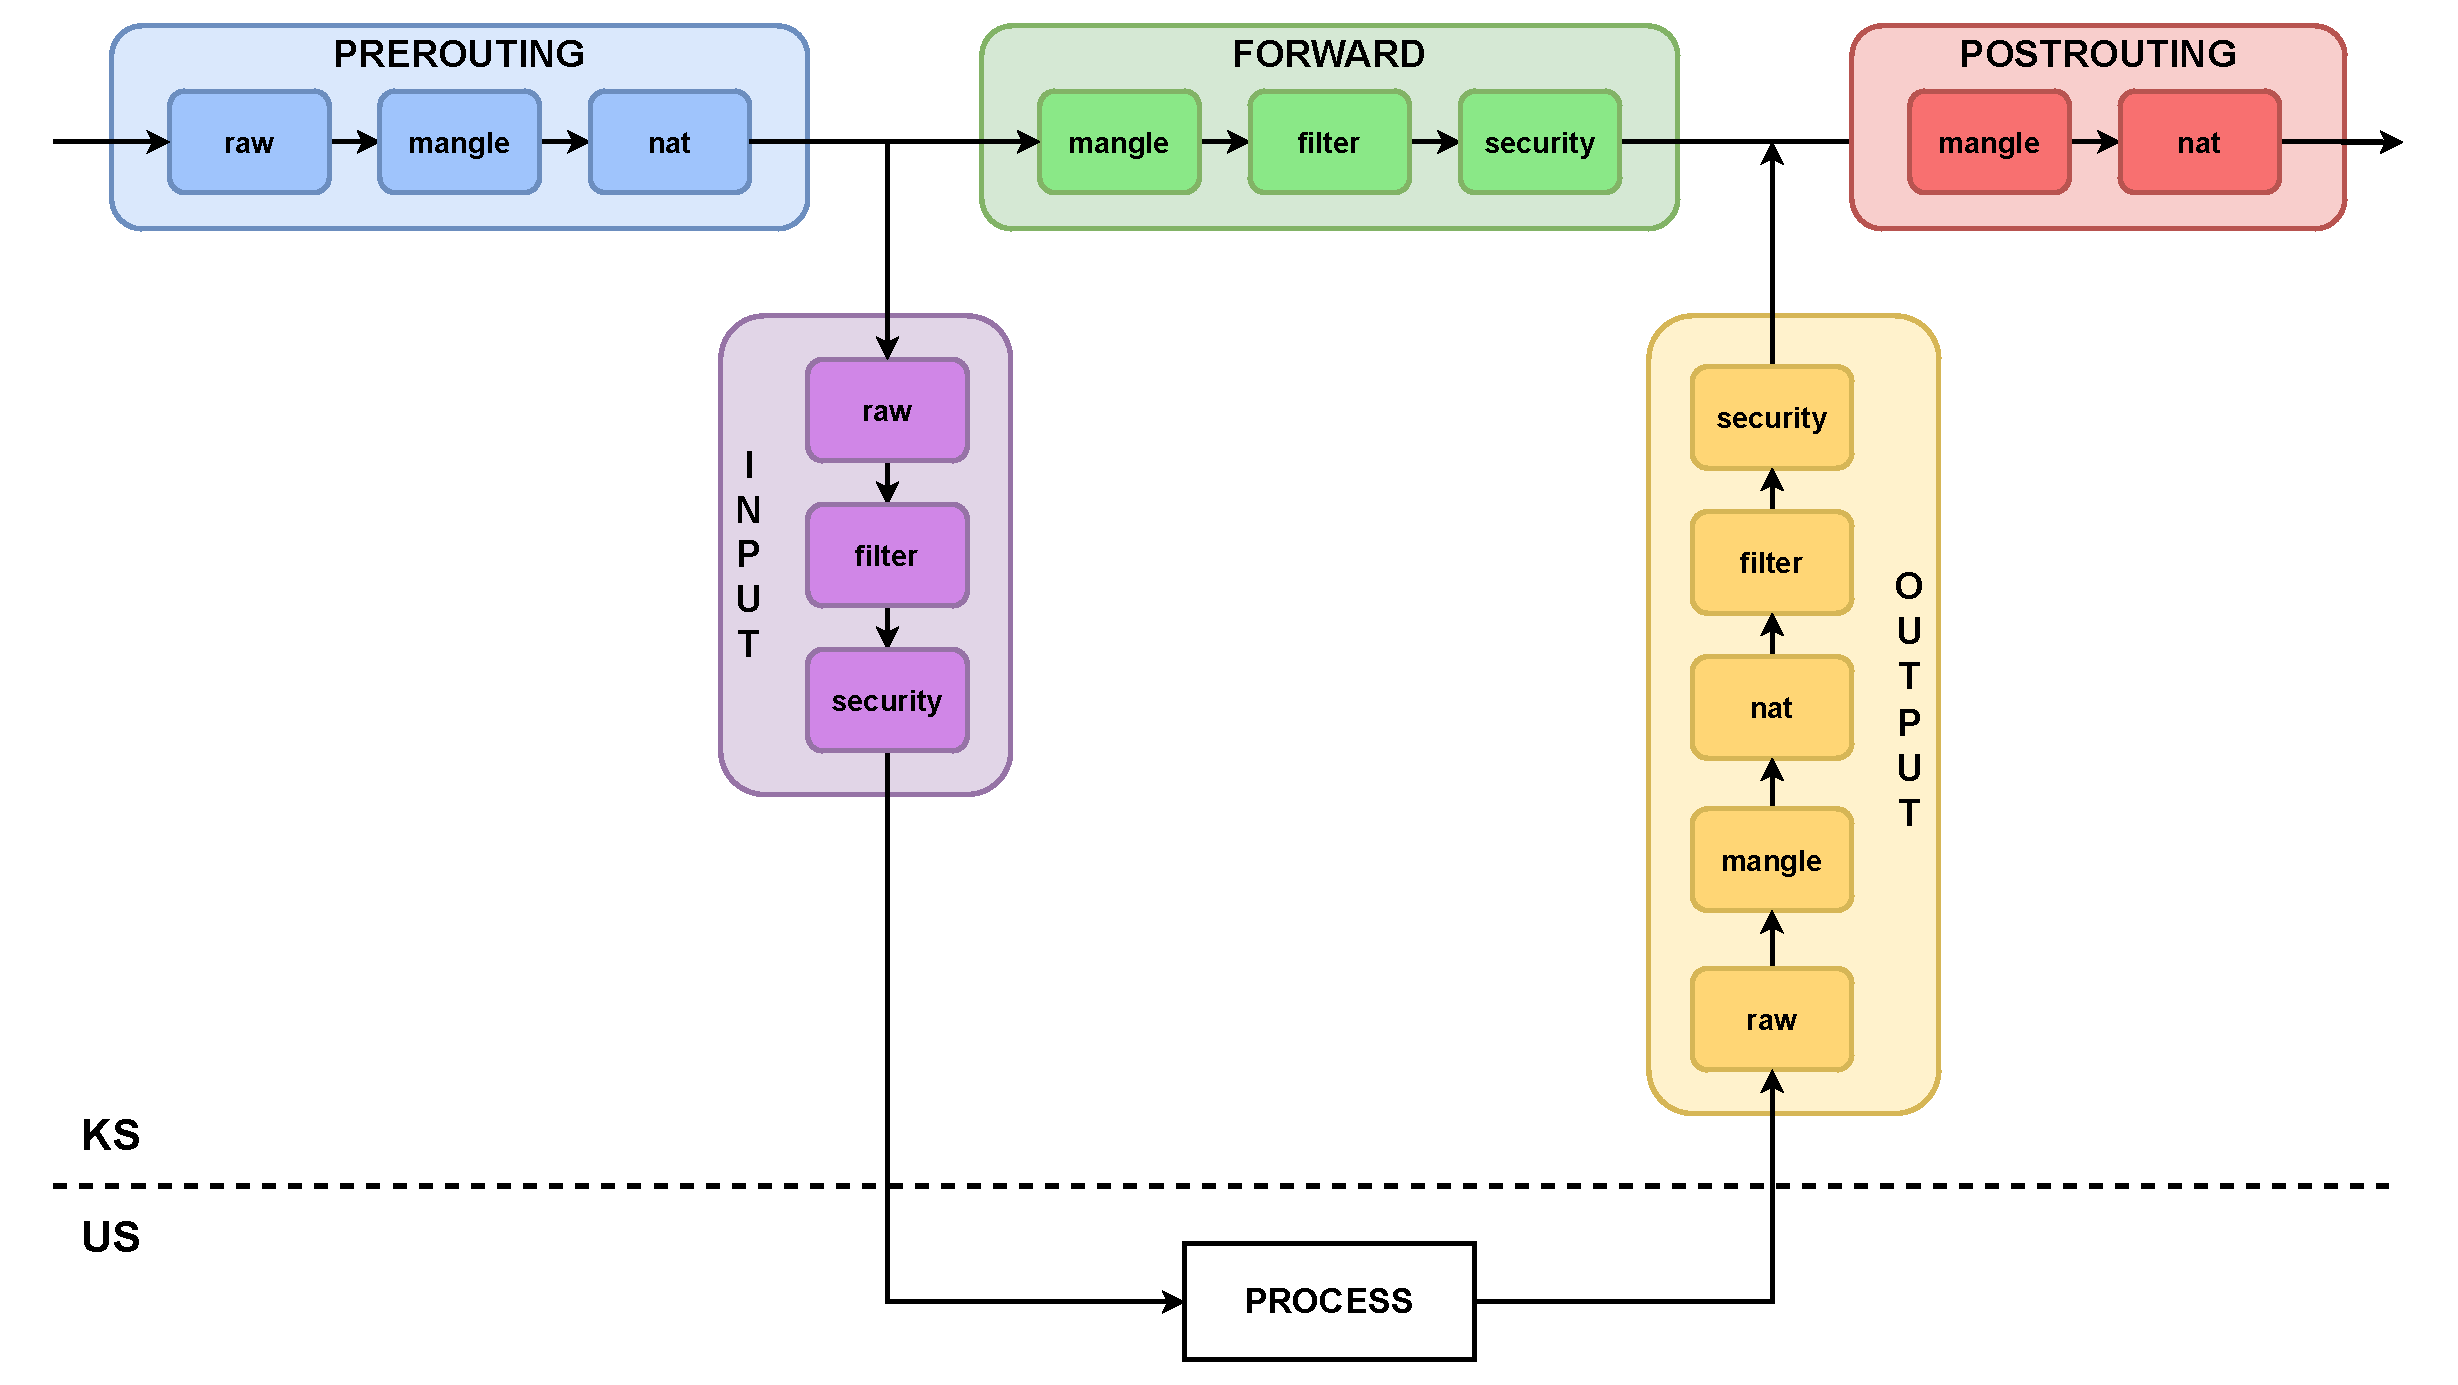
\includegraphics[width=\textwidth,keepaspectratio]{figures/netfilter_struct.pdf}
    \caption{Netfilter framework chains and table priority.}
    \label{background:firewall:fig:netfilter}
\end{figure}

Out of the five tables above, only \texttt{filter} and \texttt{security} can
contain rules that are capable of blocking network traffic. Although the use of
LSMs is discussed in this thesis, the \texttt{filter} table is the only one
of interest to us.

Each Netfilter rule consists of at least two elements: the match criteria and
the jump target (i.e., the verdict). The match criteria can be composed of
multiple conditions. These conditions can reference different elements of either
the packet itself (e.g., protocol header fields) or the session as a whole (i.e.,
the \texttt{conntrack} module). Each individual condition is implemented by
different kernel modules, so matching a packet to a Netfilter rule consists of
sequentially invoking the corresponding match function and evaluating its output
until either returns a \texttt{false} value or all conditions are exhausted.
The order in which these conditions are evaluated is decided by the userspace
tool used to configure these rules (i.e., \texttt{iptables}). \texttt{iptables}
allows to dynamically load third party modules or lesser used extensions to
the standard tool distribution. The order in which the module load flags are
specified in the command line arguments of the tool invocation determine the
order in which the match conditions are presented to the kernel and thus, the
order in which they are evaluated. This can have a significant impact on
performance.

The other component of a rule (i.e., the jump target) normally takes one of two
values on the \texttt{filter} chain: \texttt{ACCEPT} or \texttt{DROP}. However,
one of these \texttt{iptables} extensions called \texttt{Netfilter Queue} introduces
a third option: \texttt{NF\_QUEUE}. Instead of allowing the packet to pass or
dropping it on the spot, it defers the decision to a userspace process. The
packet in question is queued in the receive buffer of a Netlink socket, starting
with its Layer 3 header. The userspace process can connect to this socket,
read the packets (encapsulated in Netlink headers containing certain metadata
that are abstracted by the \texttt{Netfilter Queue} library) and analyze it in full before
reporting the same \texttt{ACCEPT} or \texttt{DROP} verdict. On Linux, this is
the preferred method of performing Deep Packet Inspection (DPI). While certain other
\texttt{iptables} modules may allow for example rudimentary string pattern
matching, this is the only way of performing DPI short of writing an \texttt{iptables}
module from scratch. Most Intrusion Prevention Systems today use this method on
Linux to intercept and analyze network traffic. Here we note one particularity
of \texttt{Netfilter Queue}. Despite its purpose, it also has the ability to
\textit{modify} traffic. As a result, a Netfilter rule can modify traffic despite
being part of the \texttt{filter} table and not in the \texttt{mangle} table. The
mechanism employed to perform the packet modification is rarely used. For this
reason, it has a number of limitations (both functional and performance related)
that we discuss at length in the following chapters.

